\subsection{metoder indenfor billedbehandling}\label{subsec:kant}
Formelt kan et billede repræsenteres som en funktion af to variable:
\begin{equation}
\begin{split}
&I: \mathbb{R}^2 \rightarrow \mathbb{R} \\
&I(x,y) = \lambda \hspace{0.5 cm} (x,y)\in \mathbb{Z^+}^2, \lambda \in [0,1] \subseteq \mathbb{R}
\end{split}
\end{equation}
hvor $\lambda$ repræsentere en billedintensitet, også kaldet pixelværdi. $\lambda$ er defineret, indenfor grænserne af billedet og er 0 udenfor, dvs.: 
$$ I(x, y) =
\begin{cases}
    \lambda, & \text{hvis } 1 \leq x \leq x_{max}, 1 \leq y \leq y_{max} \\
    0,              & \text{ellers}
\end{cases}
$$
\\
\\
En kort bemærkning bør gøres om det undersøgte billedformatet. De undersøgte billeder er af filtype JPEG og hver pixelintensitet indeholder originalt 8x3 bits information til hhv. rød, grøn og blå: $\lambda_{col} = [R,G,B]^T \in \mathbb{R}^3$. Hver farve kan antage $2^8 = 256$ værdier og hver værdi ligger i intervallet $[0,1]$. Disse værdier bliver transformeret til en gråtone værdi, vha. Lumosity metoden <cite>:
\begin{equation}
Lum(\lambda_{col}) = [0.2126, 0.7152, 0.0722] \lambda_{col} = \lambda
\label{lumosity}
\end{equation}

Hver gang pixelværdi eller billedintensitet benævnes, er det underforstået, at de har undergået den lineære transformation, ligning \cite{lumosity}. $x$ og/eller $y$ kan højst antage værdien 65.535, og et billede er derfor i sagens natur diskret.
\\
\\
Diskontinuitet i billeder er ofte en nyttig egenskab, i en billedanalytisk procedure. Det kan være i form af en kant: Hvis et billede beskues i 3D, kan en kant illustreres i 1D, ved et snit af et billede vinkelret på overfladen, illustreret figur \ref{fig:kant}. En kant er en lokal ændring i det afledte signal $f$.
\noindent
\begin{figure}[H]
    \centering
    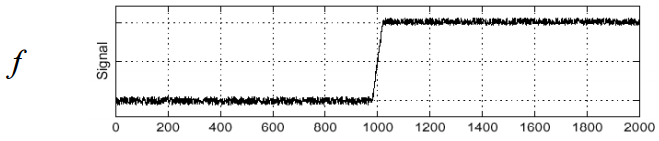
\includegraphics[width=0.55\textwidth]{fig/7.png}
     \vspace{-1em}
    \begin{center}        
     \caption{\textcolor{gray}{\footnotesize \textit{
En 1-dimensional fortolkning af intensiteten i et billede. Intensitetsskiftet i midten (x = ~1000, indikerer en kant.}}}
    \label{fig:kant}
     \end{center}
       \vspace{-2.5em}
  \end{figure}
\noindent
En differentiering af funktionen fra figur \ref{fig:kant} vil fremhæve dens udsving og derved angive hvor der forekommer kanter. Differentiering af billeder kan approsikmeres ved følgende ligning:
\begin{equation}
\dfrac{df(x)}{dx}=\dfrac{f(x+1)-f(x-1)}{2}
\label{diff}
\end{equation}
Foldning af $I$ af størrelse $(M \times N)$, med en kerne $K$ der har størrelse $(m \times n)$, hvor $M > k, N > n$:
\begin{equation}
O(i,j) = \sum\limits_{x=1}^m \sum\limits_{y=1}^n I(i+k-1,l-1)K(k,l)
\label{foldning}
\end{equation}
Ligning \eqref{foldning} sker for alle $i,j \in I$. En kerne defineres her som en matrix af arbitrær dimension - ofte $(NxN)$. En kerne foldes med et billede, for at opnå en effekt, f.eks. at glatte billedet, som er tilfældet med Gausskernen. 
\\
\\
Et billede kan differentieres, som ligning \eqref{diff}, ved brug af foldning. Først defineres en kerne til horisontal differentiering $K$, som: $K = [\frac{1}{2}, 0, \frac{1}{2}]$. Kernen foldes med billedet $I$: $I \ast K $, hvor $\ast$ udgør foldningsoperatoren.
\\
\\
I grænsetilfælde, skal en kerne foldes med et billede, hvor afstanden til kanten af billedet, er skarpt mindre, end størrelsen af kernen - dvs. der iflg ligning \eqref{foldning} ganges med et område, hvor $x < 0, y < 0$. Her gælder:


Eg. $O(1,1)$, med en kerne der har størrelse $M > m > 1$, $N > n > 1$, vil inputtet til $I$ hvor $x+k-1 < 0, l-1 < 0$, være $0$. \\
\\
Det kan være problematisk at lokalisere kanter vha. differentiering. I figur \ref{fig:kant}, ses hvordan støj i billedet(de små udsving) også vil blive fremhævet, hvilket kan resultere i fejlagtige detektioner af kanter. For at fjerne støjen, kan billedet foldes med et Gaussisk filter, hvilket er en diskret approksimering til den Gaussiske funktion. Foldning af et billede med et Gaussisk filter vil resultere i en "flydende" overgang mellem pixelværdierne og derfor glatte billedet. Den Gaussiske funktion i 2-D, hvor $ \sigma $ er standardafvigelsen af den Gaussiske fordelingen, er defineret som:
\begin{equation}
G(x,y,\sigma) = \frac{1}{2 \pi \sigma ^{2}} e^{- \frac{x^{2} + y^{2}}{2 \sigma ^{2}}}
\label{2dgaussian}
\end{equation} 
For at undgå først at glatte billedet ved at folde med et Gaussfilter, og derefter folde med et differentieringsfilter, udnyttes at foldning er en associativ operation:
\begin{equation}
\dfrac{\partial}{\partial x}(G \ast f) = (\dfrac{\partial}{\partial x}G) \ast f
\end{equation}
Her er $G$ Gausskernen, men kunne være en vilkårlig anden kerne, og $f$ et signal. \\
Foldes et differentieret 1-dimensionelt Gaussfilter med signalet fra figur \ref{fig:kant}, vil det resultere i et bakkeformet signal, hvor bakken indikere en kant. For en mere lokaliserbar kant, kan den dobbelt afledte tages, som set i figur \ref{fig:deriv}. I sidstnævnte tilfælde, kan kanten lokaliseres, hvor funktionen krydser nul.
\begin{figure}[H]
    \centering
    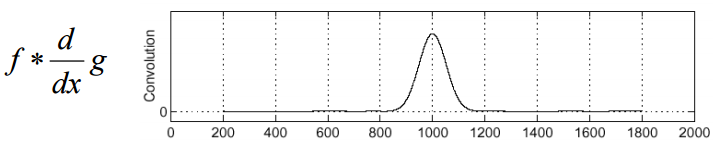
\includegraphics[width=0.55\textwidth]{fig/8.png}
    \vspace{-1em}   
    \begin{center}
    \caption{\textcolor{gray}{\footnotesize \textit{
     Resultatet af at folde et dobbelt differentieret Gaussisk filter med funktionen}}}
    \label{fig:deriv}
     \end{center}
    \vspace{-2.5em}  
  \end{figure}
\noindent
I de metoder der i denne opgave er gjort brug af, er diskontinuiteter i lokale strukturer i billederne undersøgt. Derfor er det nyttigt at bruge et dataindsamlingsvindue $\bold{D}$. Dette er en $(NxN)$ matrix af et udsnit af et billede. Givet to koordinater $(x,y)$, vil dataindsamlingsvinduet indeholde værdier der vil fremgå af konteksten, således, at $\bold{D_{\frac{N}{2},\frac{N}{2}}} = f(x,y)$, hvor $f(x,y)$ er en funktion, der er tilknyttet koordinatet $(x,y)$ i $I$ - f.eks. billedintensiteten eller en udregnet gradient.  